\documentclass{scrartcl}
\usepackage[utf8]{inputenc}
\usepackage{graphicx}
\usepackage{wrapfig}
\usepackage{listings}
\usepackage{minted}
\usepackage{subcaption}
\usepackage{csquotes}
\usepackage{hyperref}
\usepackage{amsmath}

\setlength{\parskip}{0.5em}

\title{PLSC 504: Replication Term Paper}
\subtitle{Secular Party Rule and Religious Violence in Pakistan}
\author{Mario Belledonne}
\date{\today}

\begin{document}

\maketitle

\section{Introduction}

Do terrorists cause violence in response to secular incumbency or does secular incumbency occur in response to terrorist violence?

RD in polysci


The period of $1998 \rightarrow 2003$ in Pakistan offers a "natural experiment" due to a plurality of first-past-the-post elections where both Islamist and secular leaders competed for local elections.
These elections determine the Members of the National Assembly (MNA), who are responsible for implementing local policies at the behest of their constituency.
The authors claim that secular victories within a MNA district attenuate violence at the district level, possibly moderated by police infrastructure \cite{nellis_siddiqui_2018}. 

The original authors develop a novel unit of observation (\ref{quote:joined-distict}) in an effort to mitigate geographical missmatch between the outcome variable, reports on religious violence, and treatment, secular victories. 
As a result, the authors employ a sophisticated answer strategy around these units.
In this work, I both replicate the main findings and explore the implications for this strategy in simulation that support the original findings.

\section{Design} \label{design}


The authors aim to measure the local average treatment effect (LATE) of secular victories on violence in democratic elections for close elections between secularists and Islamists.
Due to certain complexities in the construction of observed units, the usual sharp regression discontinuity design (RD) where the margin of victory acts as the running variable is not feasable.
Instead, the authors chose to employ an fuzzy RD estimation of the LATE using 2SLS under an instrumental variables (IV) approach.
In the following section, I will visit the authors' defense for this design before replicating their main findings (\ref{main_effect}).

\subsection{Data} \label{data}


\subsubsection{Units} \label{unit}
The main effect was obtained from reports from the BFRS Political Violence in Pakistan Dataset. This dataset tallied reports of political violence from a daily English-language newspaper, \textit{Dawn}. The geo-political units of these reports are in terms of administrative districts. This immediately posses a challenge to identification as administrative units do not correspond in a one-to-one fashion to MNA constituencies and have re-organized over time.

Rather than interpolating violence at the district level to the constituency level, the authors define a novel geo-political unit of analysis, \texttt{joined-district}, that clusters administrative districts into groups that contain a complete set of constituencies \ref{quote:joined-district}.

\begin{displayquote} \label{quote:joined-district}
  ...the smallest amalgamation of districts that encompasses complete MNA constituencies. 
\end{displayquote}

Importantly, the \texttt{joined-districts} have reorganized over time.
Both administrative districts and MNA constituencies where partially reorganized in 2002 (TODO cite?).
The authors note concern regarding autocorrelation of \texttt{joined-districts} that where previously members of the same unit. 
This leads to the introduction of a second unit, the \texttt{cluster districts}, that describes a second level of \texttt{joined-districts} defined as the smallest set of time-invariant administrative districts containing complete MNA constituencies between 1988 and 2013.
In other words, \texttt{joined-districts} are subsets of \texttt{cluster districts} that the authors hope would capture any control for any error correlation among units at a given election year.


\subsubsection{The Outcome Variable} \label{outcome}

The authors use a variety of outcomes for religious violence for a particular joined-district $i$ at election $t$, $Y_{i,t}$.

\begin{enumerate}
\item Any Event: A binary variable that is \textit{True} if any form of religious violence occured during the MNA's time in office for that district
\item Any Killed: Similar to \textit{Any Event} but referring to any deaths
\item Event Count: The number of religious-violent events
\item Number Killed: The number of deaths caused by religious violence
\item Number of days: The number of days in which at least one instance of religious violence occured.
\end{enumerate}

For each of these, a violent event was considered religiously motivated if there was no explicit evidence to suggest the contrary.
The authors defend this criteria by noting that the majority of religious violence is labeled as politically motivated due to the perpetrators belonging to religious political groups.
Additionally, the authors perform robustness checks by removing units in the Karachi and Balochistan provinces as those regions have a high proportion of political violence arising from non-religiously motivated assassination (TODO cite, ref result). 

\subsubsection{The Treatment Variable} \label{treatment}

As described above in \ref{quote:joined-district}, the nature of MNA constituency aggregation leads treatment, $D_{i,t} \in [0, 1]$, to take on a rational value, the proportion of MNA seats won by secularist candidates in a \texttt{joined-district}.

\subsection{Answer Strategy} \label{id}

The original authors motivate their 2SLS estimation procedure by first exploring the pitfalls of naive estimation via difference in means.

\subsubsection{Naive Estimation: Difference in Means} \label{dim}

\begin{figure}[h]
  \centering
  \scalebox{0.5}{
    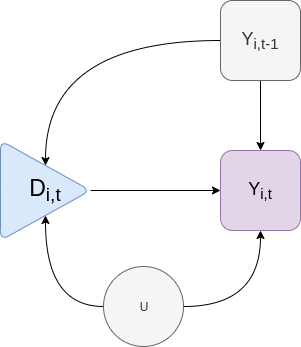
\includegraphics{replication/output/dags-ate_dim.png}
  }
  \caption{DIM Bias}
  \label{fig:ate_dim}
\end{figure}

The bivariate Difference in Means (DIM) estimator for the ATE takes the following form: 
\begin{equation} \label{eq:1}
  Y_{i,t} = \alpha + \beta * D_{i,t} + \epsilon_{i,t}
\end{equation}
Where, $D_{i,t}$ is the treatment and $\epsilon_{i,t}$ describes the error term for that unit, $(i,t)$.

Given the domain and design there are several probable sources of bias with this estimate.

\begin{enumerate}
\item  Time lagged treatment and outcomes: \texttt{joined-districts} with histories of religious violence may seek out / distrust secularists. 
\item Confounding variables: Covariates such as state capacity, education, economic stability may both impact popular opinion of secular vs religious candidates differentially
\item provincial FEs?
\item autocorrelation across temporally varying units: As mentioned in \ref{unit}, since some group of units at time $t$ to have been part of the same unit a $t-1$, it is possible for the error terms across those units to be correlated. (Note this would bias the estimate of SE)
\end{enumerate}

\subsubsection{Regression Discontinuity}
Given that at some narrow margin of victory/defeat, the probability of treatment, a secular victory, would be as if random, regression discontinuity presents itself as an appealing answer strategy for estimating an \texttt{ATE} localized around the cutoff \cite{Cattaneo_2019}. 
However as alluded to in \ref{unit} and \ref{treatment}, the aggregate nature of the data does not lend itself to a clearly identified running variable.
Given $D_{i,t}$, the proportion of secularist victories for that unit, it is not immediately clear how the aggregate (average) election margins could be interpreted as a running variable. 

\subsubsection{2SLS IV estimation} \label{iv}

The authors resort to 2SLS estimation strategy using a quasi-fuzzy RD argument.
Rather than margin of victory serving as the running variable, the authors instead define and use the proportion of secularist victories where the margin of victory was $ \leq 3\%$ as an exogenous regressor for treatment.
This exogenous regressor, $Z_{i,t}$, cannot be used as a running variable as it does not have a clear cutoff without additional assumptions.
Thus, the authors settle on instrumental variables estimation even though the instrument, in this case, covaries with treatment out of logical construction rather than causal relation.

In addition to the instrument, the authors attempt to control for unobserved covariates that would influence the proportion of close secularist victories by controlling for the proportion of close races either won or lost by secular canditates by $\leq 3\%$, $X_{i,t}$.
In the Extensions section (\ref{extensions}), I will present criticism of this answer strategy and offer alternatives revolving around binary treatment variables and single election districts.

The 2SLS answer strategy requires the following assumptions \cite{morgan_2015, Imbens_2008, Cattaneo_2019}.
For outcome ($Y_{i,t}$), treatment ($D_{i,t}$), a running variable ($Z_{i,t}$), and a cutoff $c$:
\begin{enumerate}
\item{Exogenous instrument/regressor}
\item{Non-zero first stage: $D_{i,t} \not\!\perp\!\!\!\perp Z_{i,t}$}
\item{Exclusion Restriction: $Y_{i,t} \perp Z_{i,t} \| D_{i,t}$}
\item{Monotonicity}: $Pr(D_{i,t}(Z) | Z > c) > Pr(D_{i,t}(Z) | Z < c)$
\item{Non-interference}
\end{enumerate}

The authors defend the exogeneity of the instrument by ensuring that the instrument did not predict a variety of pre-treatment covariates including state capacity, agricultural production, census data (education, utilities), and voter participation. These results are replicated in \ref{exo} along with a density test \ref{fig:density}.

The \texttt{non-zero first stage} is replicated in table \ref{table:first_stage} by calculating the first-stage regression described in eq \ref{eq:1}.

The assumption of the \texttt{exclusion restriction} is defended by the construction of their running variable.
By conditioning on the incidence of close secularist races ($X$), the only logical path that the proportion of close secular victories could effect violence would be through the proportion of victories. 
While the original work does not explicitly mentioned the assumption of \texttt{monotonicity}, this assumption is defended on similar grounds. As the proportion of close secular victories increase, so must the proportion of secular victories regardless of the margin.

\paragraph{Fixed Effects}
The original compilers of the BFRS dataset recommend using province level fixed effects, $\theta_p$ in order to control for regional differences in reporting behavior.
However, the authors note that excluding FE did not change the main estimates. (TODO add figure in results)


\begin{figure}[h]
  \centering
  \scalebox{0.5}{
    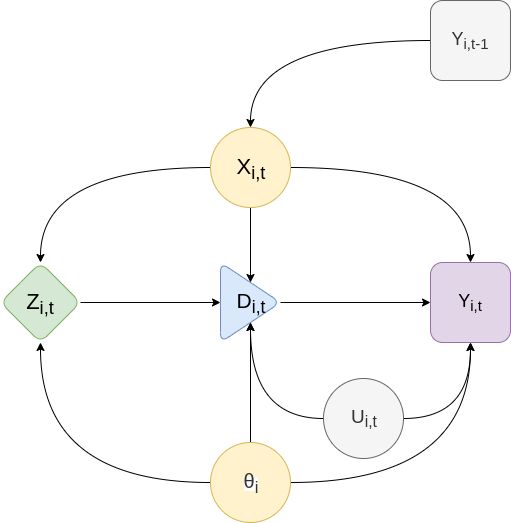
\includegraphics{replication/output/dags-ate_iv.png}
  }
  \caption{IV Model}
  \label{fig:ate_iv}
\end{figure}

In sum, figure \ref{fig:ate_iv} illustrates the model identifying the LATE.
They formally define a two stage estimation strategy as follows:

\begin{equation} \label{eq:2}
  \widehat{D_{i,t}} = \mu + \lambda * Z_{i,t} + \kappa*X_{i,t} + \theta_p + v_{i,t}
\end{equation}

 \begin{equation} \label{eq:3}
  Y_{i,t} = \alpha + \beta * \widehat{D_{i,t}} + \gamma*X_{i,t} + \theta_{p} + \epsilon_{i,t}
\end{equation}

Where

\begin{itemize}
\item $Z_{i,t}$ describes the proportion of MNA seats won by secular candidates when in close competition with Islamist candidates (within $\pm 3\%$).
\item $\widehat{D_{i,t}}$ is the predicted proportion of MNA seats won by secular candidates across all races in that district.
\item $\theta_p$ describes a geo-spatial fixed effect of violence reporting at the province level. 
\end{itemize}

Here \ref{eq:2} refers to the first stage and \ref{eq:3} refers to the estimator of the \texttt{LATE} localized to close races between secular and Islamist MNA elections.  

\begin{figure}
  \begin{subfigure}{.5\textwidth}
    \centering
    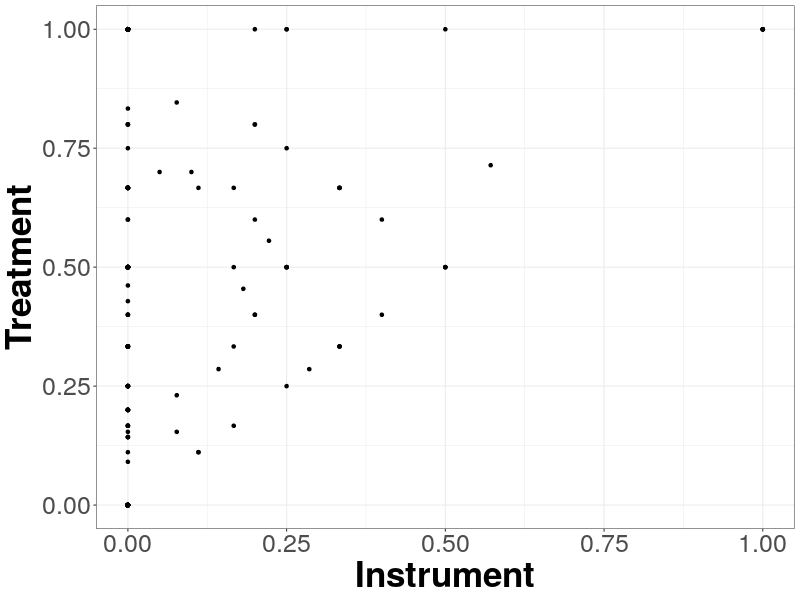
\includegraphics[width=.95\linewidth]{replication/output/D_on_Z.png}
    \label{fig:sfig1}
  \end{subfigure}%
  \begin{subfigure}{.5\textwidth}
    \centering
    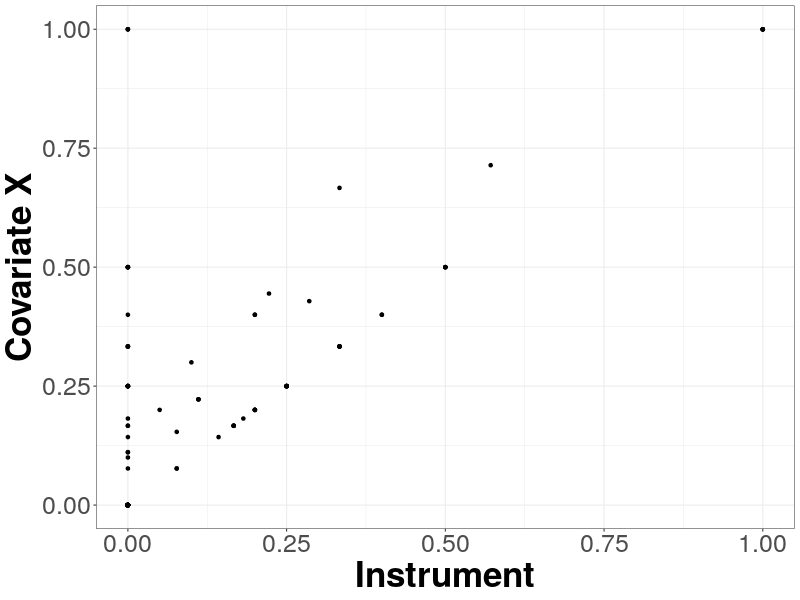
\includegraphics[width=.95\linewidth]{replication/output/X_on_Z.png}
    \label{fig:sfig2}
  \end{subfigure}
  \caption{Visualized the data}
  \label{fig:the_data}
\end{figure}


\begin{figure}
    \centering
    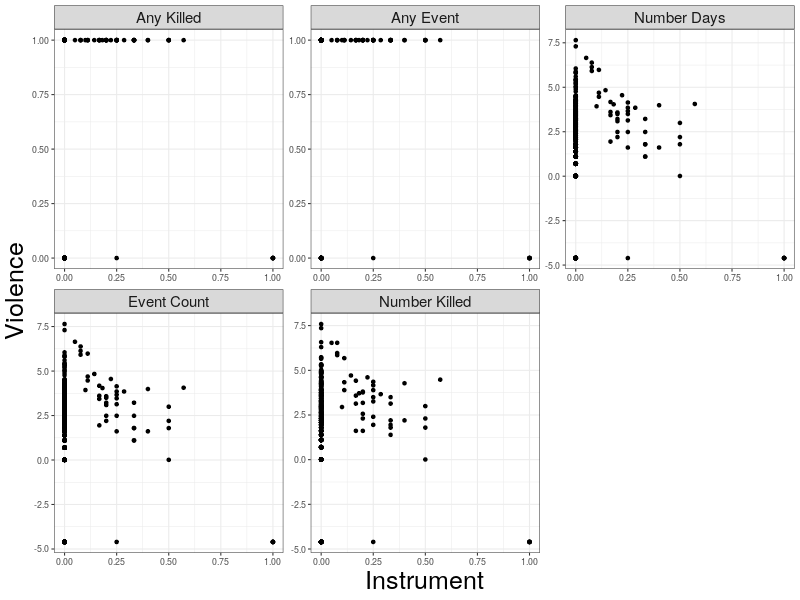
\includegraphics[width=0.8\linewidth]{replication/output/Y_on_Z.png}
    \caption{Religious Violence Across instrument}
    \label{fig:Y_on_Z}
\end{figure}

To give insight to how the outcome variables, treatment, and covariate ($X$) vary with the instrument, I visualized figure \ref{fig:the_data} \ref{fig:Y_on_Z}.

\section{Results}
\subsection{Estimates for the LATE} \label{late_results}

\begin{table}[ht]
  \begin{center}
    \scalebox{0.75}{
      
\begin{tabular}{l c c}
\hline
 & Replication & Original \\
& Any Event & \\
\hline
Prop. Secular Win        & $-0.660^{***}$  & $-0.660^{***}$\\
                         & $(0.215)$       & $(0.212)$\\
Prop. Secular Close Race & $0.031$         & $0.031$\\
                         & $(0.085)$       & $(0.084)$\\
\hline
Province FEs             & Y               & Y\\
Num. obs.                & 437             & 437\\
\hline
\multicolumn{3}{l}{\scriptsize{\parbox{.4\linewidth}{\vspace{2pt}$^{***}p<0.01$, $^{**}p<0.05$, $^*p<0.1$. \\
       Robust SEs clustered by cluster-district area, in brackets\\}}}
\end{tabular}

    }
    \caption{2SLS LATE with STATA SE estimation}
    \label{table:iv_single}
  \end{center}
\end{table}

In table \ref{table:iv_single}, we replicate the main estimate, the LATE of the proportional of seats won by secular leaders on religious violence for compliers. The full replication table is reported in \ref{table:iv_full}

\begin{table}[h!]
  \begin{center}
    \scalebox{0.75}{
      
\begin{tabular}{l c c}
\hline
 & Replication & Original \\
& Any Killed & \\
\hline
Prop. Secular Win        & $-0.477$  & $-0.477^{*}$\\
                         & $(0.296)$ & $(0.271)$\\
Prop. Secular Clost Race & $0.004$   & $0.004$\\
                         & $(0.173)$ & $(0.158)$\\
\hline
Province FEs             & Y               & Y\\
Num. obs.                & 437             & 437\\
\hline
\multicolumn{3}{l}{\scriptsize{\parbox{.4\linewidth}{\vspace{2pt}$^{***}p<0.01$, $^{**}p<0.05$, $^*p<0.1$. \\
      Robust SEs clustered by cluster-district area, in brackets\\}}}
\end{tabular}

    }
    \caption{2SLS LATE with CR2 SE estimation}
    \label{table:iv_cr2_single}
  \end{center}
\end{table}

However, it is important to note that the significance of these estimates are sensitive to the standard error estimation strategy (\texttt{stata}).
In table \ref{table:iv_cr2_single}, I recalculated the effects using \texttt{CR2} standard error estimation and the effect for \textit{Any Killed} was no longer significant. The full table is reported in \ref{table:iv_cr2}.

\paragraph{DIM estimates of ATE}

\begin{table}[h!]
  \begin{center}
    \scalebox{0.75}{
      
\begin{tabular}{l c c c c c }
\hline
 & Any Event & Event Count & Any Killed & Number Killed & Number Days \\
\hline
Secularist Close Win & $-0.176$           & $-1.265$           & $-0.141$           & $-0.769$           & $-1.265$           \\
                     & $[-0.373;\ 0.020]$ & $[-2.654;\ 0.123]$ & $[-0.331;\ 0.049]$ & $[-2.142;\ 0.605]$ & $[-2.654;\ 0.123]$ \\
\hline
R$^2$                & 0.330              & 0.393              & 0.398              & 0.390              & 0.393              \\
Adj. R$^2$           & 0.267              & 0.336              & 0.341              & 0.332              & 0.336              \\
Num. obs.            & 59                 & 59                 & 59                 & 59                 & 59                 \\
RMSE                 & 0.279              & 2.303              & 0.280              & 2.435              & 2.304              \\
\hline
\multicolumn{6}{l}{\scriptsize{Robust SEs clustered by cluster-district area, in brackets}}
\end{tabular}

    }
    \caption{Difference in Means Estimate}
    \label{table:dim}
  \end{center}
\end{table}

The authors also compute a difference-in-means (DIM) estimate of the ATE by selecting units with a single election. 
These results are replicated in table \ref{table:dim}.
To this end, the authors restrict the dataset to 59 years and joined-district points where there was a single close election between secular and Islamist candidates. I was able to replicate the original findings, with a significant negative effect for \textit{Any Event, Event Count} and \textit{Number of Days}.
Table \ref{table:dim_cr2} shows the results calculated with \texttt{CR2} standard errors. 

\subsection{Design Checks}
\paragraph{Non-zero First Stage}

\begin{table}[ht]
  \begin{center}
    \scalebox{0.85}{
      
\begin{tabular}{l c }
\hline
 & Prop. Secular Win \\
\hline
Prop. Secular Close Win  & $0.903^{***}$ \\
                         & $(0.123)$     \\
Prop. Secular Close Race & $-0.098$      \\
                         & $(0.103)$     \\
\hline
Num. obs.                & 437           \\
F statistic              & 54.446        \\
RMSE                     & 0.346         \\
\hline
\multicolumn{2}{l}{\scriptsize{\parbox{.4\linewidth}{\vspace{2pt}$^{***}p<0.01$, $^{**}p<0.05$, $^*p<0.1$. \\
       Robust SEs clustered by cluster-district area, in brackets\\ F-statistic reported for Prop.Secular Close Win}}}
\end{tabular}

    }
    \caption{First Stage Regression}
    \label{table:first_stage}
  \end{center}
\end{table}

A key component to an IV design is a non-zero first stage \ref{iv}. In other words, the exogenous instrument, $Z_{i,t}$ must have a statistically significant effect on treatment, $D_{i,t}$.
Table \ref{table:first_stage} replicates the original work where the proportion of close wins by secular candidates has a strong effect on the proportion of secular wins by any margin (eq \ref{eq:2}).

%% TODO: Explore validation of exclusion restriction
%% \paragraph{Exclusion Restriction}
%% \begin{table}[ht]
%%   \begin{center}
%%     \scalebox{0.725}{
%%       
\begin{tabular}{l c c c c c }
\hline
 & Any Event & Event Count & Any Killed & Number Killed & Number Days \\
\hline
Prop. Secular Close Win  & $-0.277$  & $12.539$  & $0.542$   & $15.823$  & $14.303^{*}$ \\
                         & $(0.684)$ & $(7.510)$ & $(0.967)$ & $(9.684)$ & $(7.984)$    \\
Prop. Secular Close Race & $-0.091$  & $-8.508$  & $-0.519$  & $-10.388$ & $-9.450^{*}$ \\
                         & $(0.386)$ & $(5.111)$ & $(0.585)$ & $(6.631)$ & $(5.502)$    \\
\hline
Num. obs.                & 437       & 437       & 437       & 437       & 437          \\
F statistic              & 9.455     & 15.030    & 4.264     & 2.639     & 14.971       \\
RMSE                     & 0.270     & 2.758     & 0.354     & 3.277     & 2.908        \\
\hline
\multicolumn{6}{l}{\scriptsize{\parbox{.4\linewidth}{\vspace{2pt}$^{***}p<0.01$, $^{**}p<0.05$, $^*p<0.1$. \\
       Robust SEs clustered by cluster-district area, in brackets\\ F-statistic reported for Prop. Secular Close Win}}}
\end{tabular}

%%     }
%%     \caption{Exclusion Restriction}
%%     \label{table:exclusion_restriction}
%%   \end{center}
%% \end{table}

\paragraph{Exogenous Instrument} \label{exo}
\begin{table}[ht]
  \begin{center}
    \scalebox{0.75}{
      
\begin{tabular}{l c c c c c }
\hline
 & Any Event & Event Count & Any Killed & Number Killed & Number Days \\
\hline
Prop. Secular Win        & $-0.066$      & $-1.165$  & $-0.127$     & $-1.404$  & $-1.162$  \\
                         & $(0.251)$     & $(1.947)$ & $(0.245)$    & $(1.969)$ & $(1.947)$ \\
Prop. Secular Close Race & $-0.364^{**}$ & $-1.802$  & $-0.313^{*}$ & $-1.696$  & $-1.811$  \\
                         & $(0.163)$     & $(1.335)$ & $(0.168)$    & $(1.398)$ & $(1.335)$ \\
\hline
Num. obs.                & 437           & 437       & 437          & 437       & 437       \\
RMSE                     & 0.301         & 2.535     & 0.355        & 2.904     & 2.540     \\
\hline
\multicolumn{6}{l}{\scriptsize{\parbox{.4\linewidth}{\vspace{2pt}$^{***}p<0.01$, $^{**}p<0.05$, $^*p<0.1$. \\
       Robust SEs clustered by cluster-district area, in brackets}}}
\end{tabular}

    }
    \caption{Placebo Check — Can Secular Victory in Close Elections at Time t Predict Prior Violence}
    \label{table:placebo}
  \end{center}
\end{table}
\begin{table}[ht]
  \begin{center}
    \scalebox{0.75}{
      
\begin{tabular}{l c c c }
\hline
 & No Fixed Effects & Disctrict Cluster FE & Disctrict Cluster + Province-Year FEs \\
\hline
Secularist Close Race & $-0.355^{***}$ & $-0.386^{***}$ & $-0.257^{***}$ \\
                      & $(0.119)$      & $(0.111)$      & $(0.091)$      \\
\hline
Num. obs.             & 437            & 437            & 437            \\
RMSE                  & 0.371          & 0.337          & 0.294          \\
\hline
\multicolumn{4}{l}{\scriptsize{\parbox{.4\linewidth}{\vspace{2pt}$^{***}p<0.01$, $^{**}p<0.05$, $^*p<0.1$. \\
       Robust SEs clustered by cluster-district area, in brackets}}}
\end{tabular}

    }
    \caption{Correlation Between Close Secular/Nonsecular Elections and Violence at Time t-1}
    \label{table:4}
  \end{center}
\end{table}

In order to address the potential influence of reverse causality, the authors attempted to predict the previous outcome for a given joined-district $Y_{i,t-1}$.
I was able to reproduce the authors' null result \ref{table:placebo}.
However, it is important to note that the instrument can predict $Y_{i,t-1}$.
The authors explore this correlation in \ref{table:4}, showing that close secular races tend to occur in low violence joined-districts.
Further analysis, shows that the instrument does not predict a variety of pre-treatment covariates such as agricultural production, education, and civil infastructure \ref{table:pretreatment_census}.

\paragraph{Monotonicity}

\begin{figure}[h]
  \centering
  \scalebox{0.5}{
    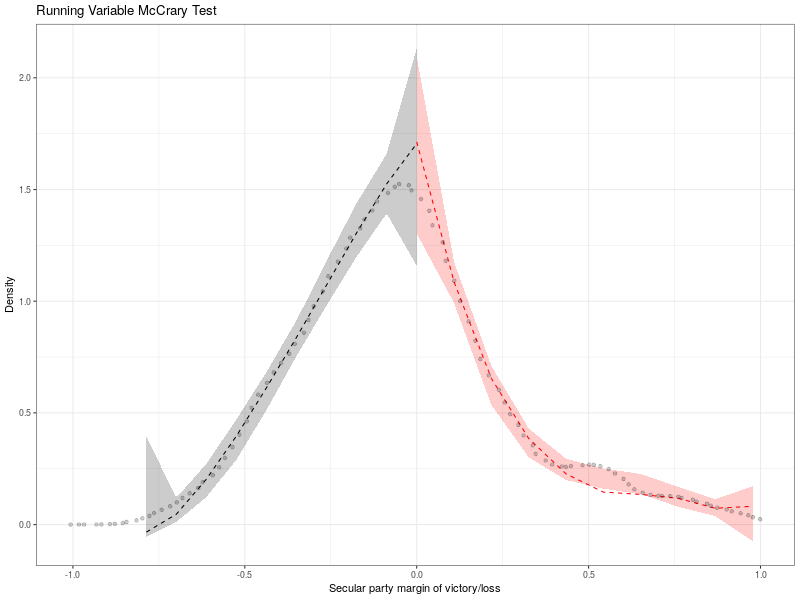
\includegraphics{replication/output/fig_a4.png}
  }
  \caption{McCrary Density Test}
  \label{fig:density}
\end{figure}
%% TODO: Add mccrary test table

In an effort to obviate concerns of sorting described in \ref{iv}, the authors perform a density test that shows a null result (fig \ref{fig:density}) \cite{mccrary_2008}.
While this cannot conclusively rule out sorting or attrition, a null result suggests that treatment is as good as random under the instrument (TODO: cite McCrary). 

\subsection{Mechanisms}

The later section of the source, the authors perform explanatory analysis to illustrate potential mechanisms of secular MNA seats on religious violence. One explored avenue was the electoral accountability. The authors claim that secular leaders often include diminished religious violence as a campaign promise. The authors then predict that secular MNA candidates expect to suffer in future elections if religious violence does occur during their tenure. 

To test their prediction, the authors estimate the causal effect of religious violence in the previous term on the proportion of secular MNA seats in the following election.
I was able to reproduce these estimates in full (table \ref{table:mechanisms})

\begin{table}[ht!]
  \begin{center}
    \scalebox{0.75}{
      
\begin{tabular}{l c c c c }
\hline
 &  &  &  &  \\
\hline
OLS                                          &                &                &               &               \\
                                             &                &                &               &               \\
\quad Prop. Secular (t-1) x Any violence     & $-0.115^{***}$ &                & $-0.102^{**}$ &               \\
                                             & $(0.040)$      &                & $(0.043)$     &               \\
\quad Prop. Secular (t-1) x Event count (ln) &                & $-0.018^{***}$ &               & $-0.014^{*}$  \\
                                             &                & $(0.006)$      &               & $(0.007)$     \\
\quad Any violence                           & $0.105^{***}$  &                & $0.086^{***}$ &               \\
                                             & $(0.028)$      &                & $(0.024)$     &               \\
\quad Prop. secularist wins (t - 1)          & $0.038$        & $-0.053^{**}$  & $0.050$       & $-0.030$      \\
                                             & $(0.043)$      & $(0.026)$      & $(0.050)$     & $(0.031)$     \\
Event count                                  &                & $0.018^{***}$  &               & $0.015^{***}$ \\
                                             &                & $(0.004)$      &               & $(0.004)$     \\
\hline
Num. obs.                                    & 344            & 344            & 344           & 344           \\
RMSE                                         & 0.139          & 0.138          & 0.126         & 0.127         \\
\hline
\multicolumn{5}{l}{\scriptsize{\parbox{.4\linewidth}{\vspace{2pt}$^{***}p<0.01$, $^{**}p<0.05$, $^*p<0.1$. \\
       Robust SEs clustered by cluster-district area, in brackets \\ Province Fixed effects omitted}}}
\end{tabular}

    }
    \caption{Mechanisms - Electoral Incentives}
    \label{table:mechanisms}
  \end{center}
\end{table}



\section{Extensions} \label{extensions}

\subsection{Fuzzy RD 2 - Electric Bugaloo}

ITT

\subsection{A case for Binary Treatment}


\section{Discussion}

\clearpage
\section{Supplementary}

\begin{table}[h!]
  \begin{center}
    \scalebox{0.75}{
      
\begin{tabular}{l c c c c c }
\hline
 & Any Event & Event Count & Any Killed & Number Killed & Number Days \\
\hline
Prop. Secular Win        & $-0.660^{***}$ & $-4.654^{**}$ & $-0.477^{*}$ & $-3.266$  & $-4.700^{**}$ \\
                         & $(0.215)$      & $(1.744)$     & $(0.275)$    & $(2.144)$ & $(1.767)$     \\
Prop. Secular Close Race & $0.031$        & $0.837$       & $0.004$      & $0.281$   & $0.947$       \\
                         & $(0.085)$      & $(0.875)$     & $(0.161)$    & $(1.276)$ & $(0.884)$     \\
\hline
Num. obs.                & 437            & 437           & 437          & 437       & 437           \\
F statistic              & 9.831          & 11.564        & 4.500        & 2.597     & 10.839        \\
RMSE                     & 0.357          & 3.025         & 0.389        & 3.194     & 3.114         \\
\hline
\multicolumn{6}{l}{\scriptsize{\parbox{.4\linewidth}{\vspace{2pt}$^{***}p<0.01$, $^{**}p<0.05$, $^*p<0.1$. \\
       Robust SEs clustered by cluster-district area, in brackets\\ F-statistic reported for Prop. Secular Win}}}
\end{tabular}

    }
    \caption{Instrumental Variable Results}
    \label{table:iv_full}
  \end{center}
\end{table}

\begin{table}[h!]
  \begin{center}
    \scalebox{0.75}{
      
\begin{tabular}{l c c c c c }
\hline
 & Any Event & Event Count & Any Killed & Number Killed & Number Days \\
\hline
Prop. Secular Win        & $-0.660^{**}$ & $-4.654^{**}$ & $-0.477$  & $-3.266$  & $-4.700^{**}$ \\
                         & $(0.229)$     & $(1.866)$     & $(0.296)$ & $(2.309)$ & $(1.892)$     \\
Prop. Secular Clost Race & $0.031$       & $0.837$       & $0.004$   & $0.281$   & $0.947$       \\
                         & $(0.086)$     & $(0.907)$     & $(0.173)$ & $(1.362)$ & $(0.916)$     \\
\hline
R$^2$                    & -0.580        & -0.486        & -0.164    & -0.169    & -0.482        \\
Adj. R$^2$               & -0.602        & -0.507        & -0.180    & -0.185    & -0.503        \\
Num. obs.                & 437           & 437           & 437       & 437       & 437           \\
RMSE                     & 0.357         & 3.025         & 0.389     & 3.194     & 3.114         \\
\hline
\multicolumn{6}{l}{\scriptsize{Robust SEs clustered by cluster-district area, in brackets}}
\end{tabular}

    }
    \caption{IV with CR2 SE estimation}
    \label{table:iv_cr2}
  \end{center}
\end{table}

\begin{table}[h!]
  \begin{center}
    \scalebox{0.75}{
      
\begin{tabular}{l c c c c c }
\hline
 & Any Event & Event Count & Any Killed & Number Killed & Number Days \\
\hline
Secularist Close Win & $-0.176^{*}$ & $-1.265^{*}$ & $-0.141$  & $-0.769$  & $-1.265^{*}$ \\
                     & $(0.095)$    & $(0.670)$    & $(0.092)$ & $(0.663)$ & $(0.670)$    \\
\hline
R$^2$                & 0.330        & 0.393        & 0.398     & 0.390     & 0.393        \\
Adj. R$^2$           & 0.267        & 0.336        & 0.341     & 0.332     & 0.336        \\
Num. obs.            & 59           & 59           & 59        & 59        & 59           \\
RMSE                 & 0.279        & 2.303        & 0.280     & 2.435     & 2.304        \\
\hline
\multicolumn{6}{l}{\scriptsize{Robust SEs clustered by cluster-district area, in brackets}}
\end{tabular}

    }
    \caption{DIM ATE with CR2 SE Estimation}
    \label{table:dim_cr2}
  \end{center}
\end{table}

\begin{table}[h!]
  \begin{center}
    \scalebox{0.65}{
      
\begin{tabular}{l c c c c c c c }
\hline
 & Area & Pacca Prop. HHs & Elecriticy & Gas & Total Literacy & Female Literacy & Primary Schools \\
\hline
Prop. Secular Win        & $0.104$   & $0.070$   & $-0.073$  & $-0.002$  & $-0.044$  & $-0.045$  & $0.000$      \\
                         & $(0.528)$ & $(0.124)$ & $(0.170)$ & $(0.028)$ & $(0.054)$ & $(0.045)$ & $(0.000)$    \\
Prop. Secular Close Race & $-0.319$  & $-0.125$  & $-0.080$  & $-0.021$  & $-0.047$  & $-0.024$  & $-0.000^{*}$ \\
                         & $(0.373)$ & $(0.084)$ & $(0.127)$ & $(0.027)$ & $(0.039)$ & $(0.036)$ & $(0.000)$    \\
\hline
Num. obs.                & 435       & 421       & 421       & 417       & 425       & 425       & 419          \\
F statistic              & 18.812    & 1192.829  & 180.434   & 1414.017  & 348.226   & 504.437   & 4.095        \\
RMSE                     & 0.844     & 0.253     & 0.263     & 0.103     & 0.125     & 0.113     & 0.000        \\
\hline
\multicolumn{8}{l}{\scriptsize{\parbox{.8\linewidth}{\vspace{2pt}$^{***}p<0.01$, $^{**}p<0.05$, $^*p<0.1$. \\
       Electoral outcomes for 1988, 1990, 1993, and 1997 are used to predict (as a falsification test) census outcomes measured in
1981; electoral outcomes for 2002 and 2008 are used to predict census outcomes measured in 1998. Sample sizes vary somewhat
across models due to missingness in some census data. Missingness is minimal and appears to be unsystematic.\\
       Robust SEs clustered by cluster-district area, in brackets\\ F-statistic reported for Prop. Secular Win}}}
\end{tabular}

    }
    \caption{Lagged Joined-District Characteristics Measured in Census of Pakistan 1981 and 1998}
    \label{table:pretreatment_census}
  \end{center}
\end{table}


\clearpage

\bibliography{main}
\bibliographystyle{plain}


\end{document}
